\section{Deep-Shallow}
\tikzstyle{na} = [baseline=-.5ex,remember picture]
\tikzstyle{nobox} = [rectangle,inner sep = 0]

\def\divsufsort{\texttt{divsufsort}\xspace}
\def\qsufsort{\texttt{qsufsort}\xspace}
\def\cache{\texttt{cache}\xspace}

Der \currentauthor{Marvin Böcker} Deep-Shallow SACA von Manzini und Ferragina aus ihrem Paper von 2004~\cite{saca:4} begann die Limitierung des Speicherverbrauches von SACAs.
Da das Suffixarray besonders bei großen Texten interessant ist, ist der Speicherbedarf möglichst stark zu begrenzen.
Das bedeutet, dass zusätzlich zu den $n$ Byte, welche durch den Eingabetext belegt werden und den $4n$ Byte, welche das fertige Suffixarray speichern (unter den Annahmen, dass in der Eingabe nur maximal 256 verschiedene Zeichen vorkommen und der Text die Länge von $2^{32}$ nicht übersteigt) nur wenig Hilfs-Speicherplatz belegt wird.
Insgesamt hat der Speicherbedarf der Suffixarray-Konstruktion also eine untere Schranke von $5n$ Byte.
\qsufsort (einer der Algorithmen, mit denen im Paper von Manzini und Ferragina vergleichen wird) benutzt beispielsweise $8n$ Byte an Speicher~\cite{saca:4}.
Allerdings gibt es seit der Veröffentlichung des Papers auch viele Algorithmen mit konstantem oder keinem zusätzlichen Speicherverbrauch, wie beispielsweise SACA-K~\cite{Nong}.

Im hier vorliegenden Algorithmus kann durch einen Parameter bestimmt werden, wie viel zusätzlicher Speicherplatz gegen ersparte Laufzeit eingetauscht wird.
Der im Paper verwendete Parameterwert kommt auf einen gesamten Speicherplatzverbrauch von $5.03n$, also bei einem Eingabetext von $100$ MiB auf $400$ MiB Suffix-Array und lediglich 3 MiB Hilfsspeicher.

Ein Nachteil des hier vorgestellten Algorithmus besteht in seiner schlechten Worst-Case-Laufzeit:
Er braucht theoretisch maximal $\mathcal O(n^2 \log n)$ Rechenschritte, um das Suffixarray zu konstruieren.
Allerdings konnten Manzini und Ferragina zeigen, dass das Verfahren in der Praxis dennoch gute Ergebnisse liefert~\cite{saca:4}.

\subsection{Überblick}

Der Deep-Shallow SA Sortieralgorithmus besteht aus drei Teilen: Bucket Sort, Shallow Sort und Deep Sort.

Bucket Sort wird einmalig zu Beginn verwendet, dann wird jeder Bucket mit Shallow Sort sortiert, und sobald die zu sortierenden Suffixe eine vorher festgelegte Größe an LCP haben, wird Deep Sort verwendet.

\begin{listing}
\begin{minted}[mathescape=true, escapeinside=||]{python}
def deep_shallow_sort(T: Text):
  Create a bucket for every character pair |$\alpha, \beta \in \Sigma$|.
  Call them |$B_{\alpha \beta}$|.

  # Sort T into the buckets by comparing only the first two
  # characters of every string. Represent the suffixes by their
  # starting indices in T.
  B := counting_sort(T)

  while (not all buckets are sorted) do:
    A := find the smallest unsorted bucket.
    shallow_sort(A, 0)
    Mark A as sorted.
\end{minted}
\caption{Einstiegspunkt des Algorithmus}
\label{ds:alg:main}
\end{listing}

\subsubsection{Teil 1: Bucket Sorting}

Die erste Stufe des Algorithmus erstellt $|\Sigma|^2$ Buckets.
Diese enthalten jeweils alle Suffixe, die mit den gleichen zwei Buchstaben anfangen.
Es gibt also für jede Buchstabenkombination $\alpha\beta$ einen Bucket $B_{\alpha\beta}$.
Allerdings muss nicht jeder Bucket Elemente enthalten.
Um die Suffixe in die Buckets zu verteilen, wird \textit{Counting Sort} verwendet.
Dazu werden alle Suffixe zuerst durchlaufen und gezählt, wieviele Elemente in jeden Bucket sortiert werden würden.
In einem zweiten Durchlauf werden dann die Buckets entsprechend befüllt.
Außerdem wird jeder Bucket als unsortiert markiert, wenn er mehr als ein Element enthält.
Die Buckets liegen sequentiell im Speicher des Suffixarrays, von links nach rechts sortiert.
Daher erhält jeder Bucket einen festen Speicherbereich, in dem seine Elemente sortiert werden müssen.
Kein Suffix muss nach diesem Schritt seinen Bucket wechseln.

In Algorithmus \ref{ds:alg:main} wird anhand eines Pseudocode der Einstiegspunkt des Algorithmus erklärt.
Um den Code einheitlich zu gestalten, sind die Kommentare auf Englisch gehalten.

\subsubsection{Teil 2: Shallow Sort}

Der Hauptteil des Algorithmus wählt immer den kleinsten, nicht-sortierten Bucket aus und sortiert ihn mittels Shallow Sorting.
Dabei wird Multikey-Quicksort verwendet, welches gut auf Strings funktioniert, welche keine langen gemeinsamen Prefixe haben~\cite{saca:4}.
Zur Erklärung siehe \cref{section:mkqs}.
Der normale MKQS-Algorithmus wird so abgewandelt, dass bei einer Vergleichstiefe größer einem Threshold automatisch abgebrochen wird und die verbleibenden Partitionen mit Deep Sort sortiert werden.

\subsubsection{Teil 3: Deep Sort}

Wird die Rekursion im Shallow Sorting zu tief, bedeutet das, dass im zu sortierenden Bucket viele Strings mit einem gemeinsamen Prefix liegen.
Daher wird ein Verfahren verwendet, welches diese Strings schnell sortieren kann.
Genauer gesagt werden drei Verfahren verwendet, je nachdem welches anwendbar ist.
Diese werden insgesamt Deep-Sorting genannt.

\begin{figure}[!h]
\centering
\newcommand{\tnode}{\node[draw,circle]}
\newcommand{\trans}{\draw[-stealth]}
\begin{tikzpicture}
\tnode (0) at (0,-1) {0};

\tnode (1a) at (4,0) {2};
\tnode (1b) at (2,-1) {1};
\tnode (1c) at (2,1) {1};

\tnode (2a) at (4,-1) {3};
\tnode (2c) at (4,-2) {4};
\tnode (2d) at (4,1) {5};

\tnode (3) at (4,-3) {1};

\trans (0) -- (1c) node[near start, above left] {a};
\trans (0) -- (1b) node[near start, above] {b};
\trans (0) -- (3) node[near start, below left] {c};

\trans (1c) -- (1a) node[midway, below left] {c};
\trans (1c) -- (2d) node[midway, above] {b(bac)};

\trans (1b) -- (2a) node[midway, above] {a(c)};
\trans (1b) -- (2c) node[midway, below left] {b(ac)};

\begin{scope}[xshift=-1cm]
\node at (6,1) {abbac};
\node at (6,0) {ac};
\node at (6,-1) {bac};
\node at (6,-2) {bbac};
\node at (6,-3) {c};
\end{scope}

\draw[-stealth] (7,0.5) -- (7,-1.5);
\node at (8, -0.5) {sortiert};
\end{tikzpicture}
\caption[Beispiel für einen Blind Trie]{Ein Beispiel für einen Blind Trie, welcher fünf Suffixe enthält. Die Kanten sind jeweils nur mit dem ersten Zeichen beschriftet. Die Zeichen in Klammern sind nur implizit gespeichert. Diese Information ist in der Zahl im nachfolgenden Knoten enthalten.}
\label{fg:blindtrie}
\end{figure}

Das so genannte \textit{Blind Sorting} verwendet einen Blind Trie (siehe Abbildung \ref{fg:blindtrie}), in welchen die Suffixe eingefügt werden.
Danach ist es einfach, den Trie in lexikografisch korrekter Reihenfolge zu durchlaufen.
Da der Trie allerdings einen relativ großen Speicherbereich belegt (36 Byte je String~\cite{saca:4}),  wird er nur bis zu $M$ zu sortierende Strings verwendet.

Wenn es mehr als $M$ Strings gibt, die es zu sortieren gilt, wird erneut \textit{Quicksort}~\cite{ternary_quicksort} verwendet, allerdings werden diesmal ganze Suffixe verglichen.
Die Rekursion beachtet außerdem $M$ und verwendet Blind Sorting, wenn die zu sortierende Menge klein genug ist.

\begin{figure}
\centering
\begin{tikzpicture}[remember picture]
\node[align=center] at (-4, 1.25) {$B_b$\\ (unsortiert)};
\node[align=right, draw] at (-4, 0) {banabas\tikz[na] \coordinate (0);\\ bas\tikz[na] \coordinate (1);\\ banabanabas\tikz[na] \coordinate (2);};

\node[align=center] at (0, 1.75) {$B_a$\\ (bereits sortiert)};
\node[align=left, draw] at (0,0) {abanabas\\ abas\\ \tikz[na] \coordinate (10);anabanabas\tikz[na] \coordinate (10b);\\ \tikz[na] \coordinate (11);anabas\tikz[na] \coordinate (11b);\\ \tikz[na] \coordinate (12);as\tikz[na] \coordinate (12b);};

\draw[-stealth] (0) -- (11);
\draw[-stealth] (1) -- (12);
\draw[-stealth] (2) -- (10);

\node[align=center] at (4, 1.25) {$B_b$\\ (sortiert)};
\node[align=left, draw] at (4, 0) {\tikz[na] \coordinate (0);banabanabas\\ \tikz[na] \coordinate (1);banabas\\ \tikz[na] \coordinate (2);bas};

\draw[-stealth] (10b) -- (0);
\draw[-stealth] (11b) -- (1);
\draw[-stealth] (12b) -- (2);

\node[align=center] (0) at (-2, -2) {Finde $B_b$\\ in $B_a$\\ (ohne b am Stringanfang)};
\node[align=center] (1) at (2, -2) {Leite relative\\ Sortierung her};

\coordinate (2) at (-2, -1);
\coordinate (3) at (2, -1);

\draw[-stealth] (0) -- (2);
\draw[-stealth] (1) -- (3);
\end{tikzpicture}
\caption[Funktionsweise von Induced Sorting]{Funktionsweise von Induced Sorting am Beispiel von \glqq banabanabas\grqq. Der linke Bucket $B_b$ (zur Vereinfachung gibt es nur Buckets für einzelne Buchstaben) soll mithilfe von $B_a$ sortiert werden. Dazu wird das LCP von allen Einträgen in $B_b$ berechnet (\glqq ba\grqq). Da \glqq a\grqq{} in \glqq ba\grqq{} enthalten ist, kann $B_a$ benutzt werden, um $B_b$ zu sortieren. Dazu wird $B_a$ durchlaufen um die Reihenfolge aller Elemente von $B_b$ zu bestimmen.}
\label{fg:induced}
\end{figure}

\subsubsection{Induced Sorting}

Diese beiden Verfahren nutzen die Struktur der zu sortierenden Strings, nämlich dass sie Suffixe sind, nicht aus.
Allerdings wird außerdem ein drittes Verfahren verwendet, welches \textit{Induced Sorting} heißt.
Dieses verwendet bereits sortierte Buckets, um eine Menge von Strings zu sortieren.
Dazu müssen die Strings ein gemeinsames Prefix haben.
Da Induced Sorting nur im Deep-Sorting verwendet wird, ist diese Bedingung gegeben.
Siehe zur Erläuterung Abbildung \ref{fg:induced}.

Dieses Sortierverfahren ist auch ohne zusätzlichen Speicherplatz möglich.
Allerdings ist es dann schwierig, die Positionen der unsortieren Strings im sortierten Bucket zu finden.
Daher wird der Text in (etwa) gleich große Segmente zerlegt und eine zusätzliche Datenstruktur gespeichert, die zu jedem Segment des Textes für das linkeste bereits sortierte Suffix speichert, in welchem Bucket es liegt, und wo es in diesem Bucket liegt.
Dadurch kann effizient überprüft werden, ob Induced Sorting verwendet werden kann.

Die Anzahl der Segmente für Induced Sorting kann durch einen Parameter $d$ eingestellt werden, da sie einen direkten Einfluss auf den Speicherplatzverbrauch des Algorithmus haben.
Im Paper verwendet wurde $d = 500$, welches zum oben genannten Speicherplatzverbrauch von $5.03n$ Byte führt.
Je nach Benchmark führen kleinere $d$ Werte (= mehr Speicherverbrauch) zu Verbesserungen der Laufzeit.
Es liegt am Benutzer, die richtige Balance zwischen Laufzeit und Speicherverbrauch zu finden.

Falls Induced Sorting nicht möglich ist, da kein passender Bucket gefunden wurde, können die anderen beiden Sortierverfahren weiterhin benutzt werden.

\subsection{Pseudocode}
Nachdem die verwendeten Verfahren grob und anschaulich erklärt wurden, wird nun am folgenden Pseudocode der Algorithmus im Detail erläutert.

Zuerst werden Buckets für jede mögliche zweistellige Buchstabenkombination erstellt, wie bereits oben beschrieben.
Diese werden nacheinander mit \texttt{shallow\_sort} sortiert.

\subsubsection{Blind Sort}
\begin{figure}
\centering
\newcommand{\tnode}{\node[draw,circle]}
\newcommand{\trans}{\draw[-stealth]}
\begin{tikzpicture}
\tnode at (0,0) (0) {0};
\tnode at (2,0.5) (1) {3};
\tnode at (2,-0.5) (2) {3};

\trans (0) -- (1) node[midway, above left] {a(bb)};
\trans (0) -- (2) node[midway, below left] {b(ba)};

\node[align=left] at (3,0.5) {abb};
\node[align=left] at (3,-0.5) {bba};

\begin{scope}[xshift=6cm]
\tnode at (0,0) (0) {0};
\tnode at (2,0.5) (1) {3};
\tnode[gray] at (2,-0.5) (2) {3};
\tnode at (4,0.5) (3) {3};
\tnode at (4,-0.5) (4) {4};

\trans (0) -- (1) node[midway, above left] {a(bb)};
\trans[gray] (0) -- (2) node[midway, below left] {b(ba)};

\trans (1) -- (3) node[midway, below left] {};
\trans (1) -- (4) node[midway, below left] {a};

\node[align=left] at (5,0.5) {abb};
\node[align=left] at (5,-0.5) {abba};
\end{scope}

\begin{scope}[yshift=-3cm]
\tnode at (0,0) (0) {0};
\tnode at (2,0.5) (1) {3};
\tnode at (2,-0.5) (2) {3};

\trans (0) -- (1) node[midway, above left] {a(aa)};
\trans (0) -- (2) node[midway, below left] {b(ba)};

\node[align=left] at (3,0.5) {aaa};
\node[align=left] at (3,-0.5) {bba};

\begin{scope}[xshift=6cm]
\tnode at (0,0) (0) {0};
\tnode at (2,0.5) (1) {1};
\tnode[gray] at (2,-0.5) (2) {3};
\tnode at (4,0.5) (3) {3};
\tnode at (4,-0.5) (4) {4};

\trans (0) -- (1) node[midway, above left] {a};
\trans[gray] (0) -- (2) node[midway, below left] {b(ba)};

\trans (1) -- (3) node[midway, above] {a(a)};
\trans (1) -- (4) node[midway, below=0.2cm] {b(ba)};

\node[align=left] at (5,0.5) {aaa};
\node[align=left] at (5,-0.5) {abba};
\end{scope}
\end{scope}

\node at (4.5,0) {$\Rightarrow$};
\node at (4.5,-3) {$\Rightarrow$};
\end{tikzpicture}
\caption{Zwei Fälle beim Einfügen in Blind Tries. Der einzufügende String ist \glqq abba\grqq. Die eingeklammerten Buchstaben sind nur implizit gespeichert.}
\label{fg:blind2}
\end{figure}

Blind Sort basiert auf Blind Tries, in welche die zu sortierenden Strings eingefügt werden.
Daraufhin kann der Baum In-Order durchlaufen werden, wodurch die Suffixe in lexikographischer Reihenfolge erhalten werden.
In Abbildung \ref{fg:blindtrie} findet sich ein beispielhafter Blind-Trie.

Ein Blind Trie besteht aus Knoten und Kanten in einer Baumstruktur, wobei jeder Knoten mindestens zwei Kinder hat.
Jede Kante ist mit einem Buchstaben beschriftet und jeder Knoten mit einem Index.
Ein Knoten entspricht dabei einer Menge von Strings, die einen gemeinsamen Prefix haben.
Die Zahl im Knoten gibt an, wie lang dieser gemeinsame Prefix ist.
Die ausgehenden Kanten zeigen dann an, welches das Zeichen ist, durch das sie sich unterscheiden.
Jedes Blatt entspricht einem Suffix, und ist durch einen Suffixindex gekennzeichnet.

Beim Einfügen wird jeder Kante gefolgt, die zum neuen String passt.
Hier kann es sein, dass keine passende Kante existiert.
Dann kann eine neue Kante eingefügt werden, die den Rest des Strings enthält (siehe Abbildung \ref{fg:blind2}, oberer Fall).
Der andere Fall wäre, dass zwar eine passende Kante existiert, der Index im folgenden Knoten allerdings zu groß ist und auch einen Teil enthält, der nicht mit dem String übereinstimmt.
Dann muss in die Kante ein Knoten eingefügt werden, der den gemeinsamen Teil vom unterschiedlichen Teil trennt (siehe Abbildung \ref{fg:blind2}, unterer Fall).
Für Details über die Datenstruktur siehe das Paper von Ferragina und Grossi~\cite{ds:blind}, sowieso das Paper von Manzini und Ferragina~\cite{saca:4}.

Da die ausgehenden Kanten jedes Knoten alphabetisch sortiert sind, sind auch die Blätter lexikographisch sortiert.
Mit einem Durchlauf des Baumes kann man an den Blättern die korrekte Sortierung ablesen.

Die Verwendung von Blind Sort ist auf ein konstantes $M$ beschränkt, da der Baum $36 M$ Byte an Speicher verbraucht.
Manzini und Ferragina wählen $M$ so, dass $M = n / 2000$.
Dadurch beschränkt sich der Speicher durch den Trie auf $9n/500$ Byte~\cite{saca:4}.

\begin{listing}[!t]
\begin{minted}{python}
def bentley_mcilroy_tq(A: Array<SuffixStartPos>):
  if |A| > 1:
    p := choose a pivot element

    # Rearrange A so, that every string in T[A[0, left)] is
    # smaller than p, every string in T[A[left, right)] is equal
    # to p and every string in T[A[right, |A|)] is greater than p.
    # This line compares entire suffixes.
    left, right := partition(A, p)

    deep_sort(A[0, left))
    deep_sort(A[right, |A|))
\end{minted}
\caption{Bentley-McIlroy ternäres Quicksort~\cite{ternary_quicksort} unter Verwendung von Deep Sorting als rekursiver Aufruf}
\end{listing}

\subsubsection{Ternäres Quicksort}
Für größere Buckets wird ternäres Quicksort verwendet.
Dieses sortiert den Bucket mit simplen, direkten Vergleichen über die gesamten Suffixe.
Es ist zu beachten, dass die mittlere Partition (\glqq =\grqq) nur ein Element enthält, welches \texttt{p} ist.
Daher muss diese Partition nicht sortiert werden.
Statt einem rekursiven Aufruf an sich selbst wird jedoch wieder \texttt{deep\_sort} aufgerufen, um von Blind Sort zu profitieren, falls die Partition nun klein genug ist.
Für Details über ternäres Quicksort siehe Abschnitt~\ref{section:ternary_quicksort} oder auch das Paper von Bentley und McIlroy~\cite{ternary_quicksort}.

\subsubsection{Induced Sorting}
Die bisher vorgestellten Algorithmen verwenden keine Information darüber, dass es sich bei den sortierten Strings um Suffixe des selben Textes handelt.
In diesem Abschnitt wird das Verfahren um einen Algorithmus ergänzt, welcher eine Menge von Strings sortieren kann, die ein gemeinsames Prefix haben.

Induced Sorting benutzt die bereits sortierten Buckets, um zu sortieren.
In Abbildung \ref{fg:induced} findet sich eine Visualisierung.
Die Vorraussetzung dafür ist, dass die Strings in A einen gemeinsamen Prefix haben, und dass es einen dazu passenden Bucket gibt.
Zuerst wird das eigentliche Prinzip erklärt und danach eine Verbesserung eingeführt, die die Performance auf Kosten von zusätzlichem Speicher erhöht.

Um heraus zu finden, ob Induced Sorting verwendet werden kann, wird der LCP berechnet und jeder Bucket, der in Frage kommt, überprüft.
Wenn im LCP der Strings eine zweistellige Zeichenkette $\alpha\beta$ vorkommt, für die der Bucket $B_{\alpha\beta}$ bereits sortiert wurde, so kann die Sortierung der Strings leicht aus der Ordnung des Buckets hergeleitet werden.
Alle Zeichen vor $\alpha\beta$ werden abgeschnitten.
Die so erhaltenen Strings werden im Bucket gesucht und markiert.
Dann wird der Bucket in richtiger Reihenfolge durchlaufen und jeder markierte String in dieser Reihenfolge gespeichert.
Da der Bucket sortiert war, sind folglich auch die Strings danach sortiert.

\begin{listing}[!t]
\begin{minted}{python}
def induced_sort(A: Array<SuffixStartPos>, t: Integer,
                      B: Bucket):
  n_marked := 0
  for b in B do:
    # We need to ignore the first t characters.
    if (A + t) contains b:
      Mark b in B.
      n_marked++

    if n_marked == |A|:
      Pass over B and store the marked elements to A.
      Unmark every element of B.
      return
\end{minted}
\caption{Induced Sorting, Version 1~\cite{saca:4}}
\end{listing}

\begin{figure}[!b]
\centering
\begin{tikzpicture}[remember picture]
\node at (0,0) {b\tikz[na] \coordinate[yshift=-2pt] (a);an|\tikz[na] \coordinate[yshift=-2pt] (b);aba|n\tikz[na] \coordinate[yshift=-2pt] (c);ab|\tikz[na] \coordinate[yshift=-2pt] (d);as};

\begin{scope}[xshift=-0.3cm]
\coordinate[fill, circle, inner sep = 2pt] (0) at (-0.2,-1);
\coordinate[fill, circle, inner sep = 2pt] (1) at (0.2,-1);
\coordinate[fill, circle, inner sep = 2pt] (2) at (0.6,-1);
\coordinate[fill, circle, inner sep = 2pt] (3) at (1,-1);

\draw (-0.4, -1.2) -- (1.2,-1.2) -- (1.2,-0.8) -- (-0.4,-0.8) -- cycle;
\draw (0, -1.2) -- (0,-0.8);
\draw (0.4, -1.2) -- (0.4,-0.8);
\draw (0.8, -1.2) -- (0.8,-0.8);
\end{scope}

\draw[-stealth] (0) -- (a);
\draw[-stealth] (1) -- (b);
\draw[-stealth] (2) -- (c);
\draw[-stealth] (3) -- (d);

\begin{scope}[yshift=-2.5cm]
\node at (3,1.5) {$B_a$ (sortiert)};
\node[align=left,draw] at (3,0) {\tikz[na] \coordinate (z2);abanabas\\ \tikz[na] \coordinate (z0);abas\\ \tikz[na] \coordinate (z1);anabanabas\\ anabas\\ \tikz[na] \coordinate (z3);as};
\end{scope}

\draw[-stealth] (0) |- (z1);
\draw[-stealth] (1) |- (z2);
\draw[-stealth] (2) |- (z0);
\draw[-stealth] (3) |- (z3);

\end{tikzpicture}
\caption{Verwendung der Arrays \texttt{Offset} und \texttt{Anchor} am Beispiel der Eingabe \glqq banabanabas\grqq. Die Eingabe wird in vier Segmente aufgeteilt und zu jedem Segment ein \texttt{Offset} und ein \texttt{Anchor} gespeichert. Das \texttt{Offset} entspricht jeweils dem Zeiger in den Eingabetext (oben). Der \texttt{Anchor} zeigt auf die Position dieses Suffix in seinem Bucket.}
\label{fg:offset}
\end{figure}

Die zeitintensivste Aufgabe ist laut Profiling, einen passenden Bucket zu finden~\cite{saca:4}.
Daher wird durch eine Verbesserung zusätzlicher Speicherplatz verwendet, um zwei Arrays anzulegen, \texttt{Offset} und \texttt{Anchor}.
Der Eingabetext wird in etwa gleich große Teile segmentiert.
Die Segmentgröße ist dabei durch den Parameter $d$ einstellbar.
Durch $n/d$ ergibt sich die Anzahl der Segmente.

In \texttt{Offset[i]} wird der linkeste (also kleinste) Suffix-Startindex gespeichert, der zu einem Bucket gehört, der bereits als sortiert markiert ist.
Der Wert ist dabei relativ zum Segmentbeginn.
In \texttt{Anchor[i]} wird dann die Position vom Suffix \texttt{Offset[i]} in seinem Bucket gespeichert.
In Abbildung \ref{fg:offset} findet sich eine Veranschaulichung der beiden Arrays.

Da man die Startposition von Segment \texttt{i} nicht speichern muss (da jedes Segment $i$ das Intervall $[i\cdot d, (i + 1) \cdot d]$ umfasst), und jedes Segment höchstens $d$ Elemente enthält, ist \texttt{Offset[i]} $< d$.
Unter der Annahme $d < 2^{16}$ kann man \texttt{Offset[i]} in 2 Byte speichern.
Da \texttt{Anchor[i]} die Position im Bucket enthält, und der Bucket im Worst-Case alle Suffixe enthält, sind dort die vollen $4$ Byte nötig.
Daher hat diese Erweiterung einen zusätzlichen Speicherbedarf von $6n/d$ Byte.

\begin{listing}
\begin{minted}{python}
def induced_sort(A: Array<SuffixStartPos>, t: Integer,
                      B: Bucket):
  for a in A do:
    s := a mod d # Suffix a is from this segment number.
    if a < offset[s] <= a + L:
      bucket_pos = anchor[s]
      Induce sorting like above by scanning around bucket_pos.
      return

  # If no induced sorting is possible, use other methods.
  Use Deep Sorting without Induced Sorting.
\end{minted}
\caption{Induced Sorting, Version 2~\cite{saca:4}}
\label{ds:alg:induced2}
\end{listing}

Der Algorithmus verwendet \texttt{Offset} und \texttt{Anchor} (so genannte Anker), um einen passenden, bereits sortierten Bucket und die Position in jenem Bucket zu finden.
In Algorithmus \ref{ds:alg:induced2} findet sich Pseudocode des Verfahrens.
Einer der zu sortierenden Strings wird ausgewählt und der Index des Segments berechnet.
Wenn der Eintrag von \texttt{Offset[s]} zwischen \texttt{a} und \texttt{a + L} liegt, ist klar, dass das Suffix an Position \texttt{Offset[s]} nach \texttt{a} beginnt und innerhalb der \texttt L ersten Zeichen liegt.
Daher hat es mindestens ein übereinstimmendes Zeichen an vorderster Position mit den zu sortierenden Strings.
Da bekannt ist, dass alle Strings in A die selben Zeichen an den ersten \texttt{L} Stellen haben, reicht es aus, einen der Strings aus A zu vergleichen.
Daher kann der Bucket um \texttt{Anchor[s]} nach den zu sortierenden Strings gescannt werden.
Da wir annehmen, dass die Strings im sortierten Bucket nah beieinander liegen, verbessert dies die Laufzeit~\cite{saca:4}.

\begin{figure}
\centering
\begin{tikzpicture}[remember picture]
\node at (0,0) {b\tikz[na] \coordinate[yshift=-2pt] (a);anaba};
\node at (1.3,0) {n\tikz[na] \coordinate[yshift=-2pt] (b);abas};

\node at (0,-1) (0) {1};
\node at (1.3,-1) (1) {1};
\node at (0,-1.6) (2) {2};
\node at (1.3,-1.6) (3) {1};

\draw (-0.2, -1.3) -- (0.2, -1.3);
\draw (1.1, -1.3) -- (1.5, -1.3);

\draw (-0.2, -0.7) -- (0.2, -0.7) -- (0.2, -1.9) -- (-0.2, -1.9) -- cycle;
\draw (1.1, -0.7) -- (1.5, -0.7) -- (1.5, -1.9) -- (1.1, -1.9) -- cycle;

\draw[-stealth] (0) -- (a);
\draw[-stealth] (1) -- (b);

\begin{scope}[yshift=-2.5cm, xshift=1cm]
\node at (3,1.5) {$B_a$ (sortiert)};
\node[align=left,draw] at (3,0) {\tikz[na] \coordinate (z2);abanabas\\ \tikz[na] \coordinate (z0);abas\\ \tikz[na] \coordinate (z1);anabanabas\\ anabas\\ \tikz[na] \coordinate (z3);as};
\end{scope}

\begin{scope}[yshift=-2.5cm, xshift=-6cm]
\node at (3,1.5) {$B_b$ (unsortiert)};
\node[align=left,draw] at (3,0) {banabas\\ bas\\ banabanabas};
\end{scope}

\draw[-stealth] (3) |- (z0);
\draw[-stealth] (2) |- (z1);

\end{tikzpicture}
\caption{Ausgangs-Szenario im Beispiel. Betrachtet wird der String \glqq banabanabas\grqq, und der Bucket $B_a$ ist bereits sortiert. $B_b$ soll mittels Induced Sorting sortiert werden.}
\label{fg:beispiel}
\end{figure}

Zur Veranschaulichung folgt ein kurzes Beispiel. Unser Text sei wieder \glqq banabanabas\grqq.
Sagen wir wieder, wir wollen die Strings \glqq banabas\grqq, \glqq bas\grqq{} und \glqq banabanabas\grqq{} sortieren.
Diese haben jeweils die Suffix-Indices 4, 8 und 0.
Die Länge des LCP dieser Strings ist 2 (\glqq ba\grqq).
Daher sei für dieses Beispiel $L = 2$.
Zum Sortieren benutzen wir den Bucket $B_a$, welcher bereits sortiert ist (siehe Abbildung \ref{fg:beispiel}).
Sei für dieses Beispiel $d = 6$.
Dann ist also ist jedes Segment 6 Suffixe groß und es gibt zwei Segmente.
Die Segmente sind also \glqq banaba\grqq{} und \glqq nabas\grqq.
Dann ist \texttt{Offset[0] = 1} (\glqq anabanabas\grqq) und \texttt{Offset[1] = 1} (\glqq abas\grqq).
Die jeweiligen Anker zeigen auf die Position dieser Suffixe in ihren Buckets.

Wir wählen einen der zu sortierenden Strings aus, z.B. den ersten.
Dieser hat Suffix-Index 4 und gehört daher zu Segment 0.
Da \texttt{Offset[0] == 1} und $1 \not \in [4, 4 + L]$ liegt, ist dieser Anker nicht geeignet, um die Strings zu sortieren.

Eigentlich ginge das Sortieren mittels \glqq banabas\grqq{} natürlich, da nach Löschen des ersten Zeichens \glqq anabas\grqq{} in $B_a$ liegt ($4 < 5 \leq 6$).
Um jedoch die Laufzeit gering zu halten, da nicht bekannt ist, an welcher Position \glqq anabas\grqq{} steht, werden stattdessen die anderen Kandidaten ausprobiert:

Das Segment vom zweiten String mit Suffixindex 0 ist ebenfalls 0.
Da \texttt{Offset[0] == 1} liegt 1 in diesem Fall im Intervall $[0, 0 + L] = [0, 2]$ und wir können \texttt{Anchor[0]} benutzen, um die Strings zu sortieren.
Dazu verwenden wir den Zeiger \texttt{Anchor[0]}, welcher auf die Position von \glqq anabanabas\grqq{} in $B_a$ zeigt.
Wir schneiden die ersten $(1 - 0) = 1$ Zeichen aus unserer String-Menge ab und suchen die Suffixe im Bucket, wie oben beschrieben.
Da wir bereits ein Element im Bucket kennen, und annehmen, dass die anderen Suffixe nah daran liegen, fällt das Suchen des ersten Elements im Bucket weg.
Im Ausgangspaper konnten die Autoren eine signifikante Performance-Erhöhung mittels dieses Ansatzes zeigen.

\begin{figure}[!t]
\centering
\begin{tikzpicture}[remember picture]
\node at (0,0) {\tikz[na] \coordinate[yshift=-2pt] (a);banaba};
\node at (1.3,0) {n\tikz[na] \coordinate[yshift=-2pt] (b);abas};

\node at (0,-1) (0) {0};
\node at (1.3,-1) (1) {1};
\node at (0,-1.6) (2) {5};
\node at (1.3,-1.6) (3) {1};

\draw (-0.2, -1.3) -- (0.2, -1.3);
\draw (1.1, -1.3) -- (1.5, -1.3);

\draw (-0.2, -0.7) -- (0.2, -0.7) -- (0.2, -1.9) -- (-0.2, -1.9) -- cycle;
\draw (1.1, -0.7) -- (1.5, -0.7) -- (1.5, -1.9) -- (1.1, -1.9) -- cycle;

\draw[-stealth] (0) -- (a);
\draw[-stealth] (1) -- (b);

\begin{scope}[yshift=-2.5cm, xshift=1cm]
\node at (3,1.5) {$B_a$ (sortiert)};
\node[align=left,draw] at (3,0) {\tikz[na] \coordinate (z2);abanabas\\ \tikz[na] \coordinate (z0);abas\\ \tikz[na] \coordinate (z1);anabanabas\\ anabas\\ \tikz[na] \coordinate (z3);as};
\end{scope}

\begin{scope}[yshift=-2.5cm, xshift=-6cm]
\node at (3,1.5) {$B_b$ (sortiert)};
\node[align=left,draw] at (3,0) {banabanabas\tikz[na] \coordinate (y1);\\ banabas\\ bas};
\end{scope}

\draw[-stealth] (2) |- (y1);
\draw[-stealth] (3) |- (z0);

\end{tikzpicture}
\caption{Szenario nach einem Aufruf von Induced Sorting. Der Bucket $B_b$ wurde sortiert und \texttt{Offset} und \texttt{Anchor} aktualisiert. Es ist zu beachten, dass \texttt{Anchor[0]} nun 5 ist, da dies die Position des Suffix im Speicher ist und die Buckets nacheinander im Speicher liegen. Daher beginnt die Nummerierung der Suffixe in $B_b$ dort, wo $B_a$ endet.}
\label{fg:beispiel2}
\end{figure}

Im vorherigen Abschnitt haben wir für das Beispiel angenommen, dass alle \texttt{Anchor}-Pointer auf den selben Bucket zeigen.
Das ist in der Praxis unwahrscheinlich, wodurch die Auswahl möglicher Anker weiter eingeschränkt wird.
Falls dennoch mehrere Anker zur Auswahl stehen, wird derjenige dusgewählt, der \texttt{Anchor[i mod d] - i} minimiert (also einen möglichst kurzen gemeinsamen Prefix mit dem Anker hat).

Manzini und Ferragina haben in ihren Benchmarks verschiedene Werte der Segmentgröße $d$ zwischen 500 und 5000 getestet.
Auf einigen Problemen hat eine Vergrößerung von $d$ keinen merklichen Unterschied in der Laufzeit gebracht.
Allerdings wurde die Laufzeit auf einigen Dateien dann deutlich schlechter.
Die Autoren bewerben ihren Algorithmus allerdings mit $5.03n$ Byte Speicherverbrauch, was einem $d = 500$ entspricht.

\subsection{Beispiel}

\begin{figure}[!h]
\centering
\begin{tabular}{|c|c|c|c|c|c|c|c|c|c|c|c|c|c|}
\hline
2 & 12 & 10 & 1 & 13 & 8 & 4 & 7 & 3 & 9 & 5 & 11 & 6 & 0 \\
\hline
\multicolumn{8}{|c|}{$B_a$} & \multicolumn{2}{c|}{$B_b$} & \multicolumn{4}{c|}{$B_c$} \\
\hline
\end{tabular}
\caption{SA nach Schritt 1: Counting Sort}
\label{ds:beispiel1}
\end{figure}

\newcommand{\tnode}{\node[draw,circle]}
\newcommand{\trans}{\draw[-stealth]}
\begin{figure}[!h]
\centering
\begin{tikzpicture}
\tnode at (0,0) (0) {0};
\tnode at (2,1) (1) {2};
\tnode at (2,-1) (2) {8};
\node at (4,1) {aa};
\node at (4,-1) {caabacaa};
\trans (0) -- (1) node[midway, above] {a};
\trans (0) -- (2) node[midway, below] {c};
\end{tikzpicture}
\caption{Blind Trie in der ersten Deep Sorting Phase}
\label{ds:beispiel_bt1}
\end{figure}

Zur Verdeutlichung und Veranschaulichung des Algorithmus wird im folgenden Abschnitt der Algorithmus beispielhaft\footnote{Insbesondere wird der Algorithmus mit Beispiel-Parameterwerten ausgeführt, die in einer echten Anwendung sehr unangebracht wären. Diese Parameter sind $L = 3, d = 7$.} am Eingabetext \glqq caabaccaabacaa\grqq{} ausgeführt.

\paragraph{Schritt 1} Sortiere alle Suffixe mittels Counting Sort nach dem ersten Zeichen\footnote{Sowohl die Referenzimplementierung als auch unsere Implementierung benutzen Buckets, welche nach den ersten beiden Zeichen sortiert wurden.
Aus Gründen der Veranschaulichung wird hier allerdings nach nur einem Buchstaben sortiert.} in einen der Buckets.
Der Status des Algorithmus nach diesem Schritt ist in \cref{ds:beispiel1} abgebildet.

\paragraph{Schritt 2} Sortiere alle Buckets mit Shallow Sort in nach Größe aufsteigender Reihenfolge.
Der kleinste Bucket ist $B_b$.
Dieser enthält \glqq bacaa\grqq{} und \glqq bacaa\grqq.
Wir vergleichen die Strings in MKQS bis zum dritten Zeichen.
Da wir bis dahin noch keinen Unterschied festgestellt haben, schalten wir auf Deep Sorting um. 
Weil der Bucket klein genug ist (und damit das Beispiel interessant ist), wird Blind Sorting benutzt, um den Bucket zu sortieren.
Der Blind Trie ist in \cref{ds:beispiel_bt1} dargestellt.
Beim Vergleich sind die ersten drei Zeichen ignoriert worden, da sie als gleich bekannt sind.

\begin{figure}
\centering
\begin{tikzpicture}
\tnode at (0,0.5) (0) {0};
\tnode at (2,1) (1) {0};
\tnode at (2,0) (2) {3};
\tnode at (4,0) (3) {5};
\tnode at (4,-1) (4) {11};
\node at (3,1) {\$};
\node at (6,0) {bacaa};
\node at (6,-1) {baccaabacaa};
\trans (0) -- (1) node[midway, above] {\$};
\trans (0) -- (2) node[midway, below] {c};
\trans (2) -- (3) node[midway, above] {a};
\trans (2) -- (4) node[midway, below] {c};
\end{tikzpicture}
\caption{Blind Trie in der zweiten Deep Sorting Phase}
\label{ds:beispiel_bt2}
\end{figure}

\paragraph{Schritt 3} Der Bucket $B_b$ wird als sortiert markiert und der nächstgrößere sortiert.
$B_c$ wird sortiert.
Dieser enthält \glqq ccaabacaa\grqq, \glqq caa\grqq, \glqq caabacaa\grqq{} und \glqq caabaaccaabacaa\grqq.
Beim Versuch, diese mit MKQS zu sortieren, kann nur die relative Ordnung von \glqq ccaabacaa\grqq{} und den anderen drei Suffixen hergeleitet werden: \glqq ccaabacaa\grqq{} ist größer als die anderen drei Suffixe.
Die anderen drei Suffixe haben ein zu langes LCP um komplett in Shallow Sort sortiert zu werden.
Daher wird für diese wieder ein Blind Trie benutzt, welcher in \cref{ds:beispiel_bt2} dargestellt ist.

%\paragraph{Schritt 4} Da es für den nächsten Schritt interessant sein wird, aktualisieren wir für diesen Bucket die \texttt{OFFSET-} und \texttt{ANCHOR}-Pointer.
%Für dieses Beispiel wird der Eingabetext in Segmente der Größe 7 eingeteilt.
%Als \texttt{OFFSET} wird für das linke Segment ein Pointer auf \glqq caabaccaabacaa\grqq gespeichert.
%Der rechte \texttt{OFFSET}-Pointer zeigt auf \glqq bacaa\grqq.
%Die beiden \texttt{ANCHOR}-Pointer zeigen auf die Position des jeweiligen Suffix im SA.
%Damit sind die Pointer aktuell.

\paragraph{Schritt 5} Der letzte zu sortierende Bucket, $B_c$ wird auch wieder mit Shallow Sort sortiert.
Allerdings kann durch den Vergleich der ersten drei Zeichen nicht die Ordnung von \glqq abaccaabacaa\grqq, \glqq abacaa\grqq, \glqq aabaccaabacaa\grqq{} und \glqq aabacaa\grqq{} hergeleitet werden.
Für jeweils Paare aus zwei Suffixen (\glqq aabacaa\grqq{} und \glqq aabaccaabacaa\grqq, und \glqq abaccaabacaa\grqq{} und abacaa) können wir allerdings Induced Sorting benutzen:
Im bekannten LCP der ersten beiden Strings \glqq aab\grqq{} befindet sich ein \glqq b\grqq.
Daher können wir zur Sortierung den bereits sortierten $B_b$-Bucket verwenden.
Darin suchen wir \glqq bacaa\grqq{} und \glqq baccaabacaa\grqq{} und können daraus die relative Sortierung herleiten.
Das gleiche Verfahren wird für das zweite Paar verwendet.

Schlussendlich ist damit der gesamte Text sortiert, da es keine unsortierten Buckets mehr gibt.

\subsection{Vergleich}
\begin{figure}[!h]
\centering
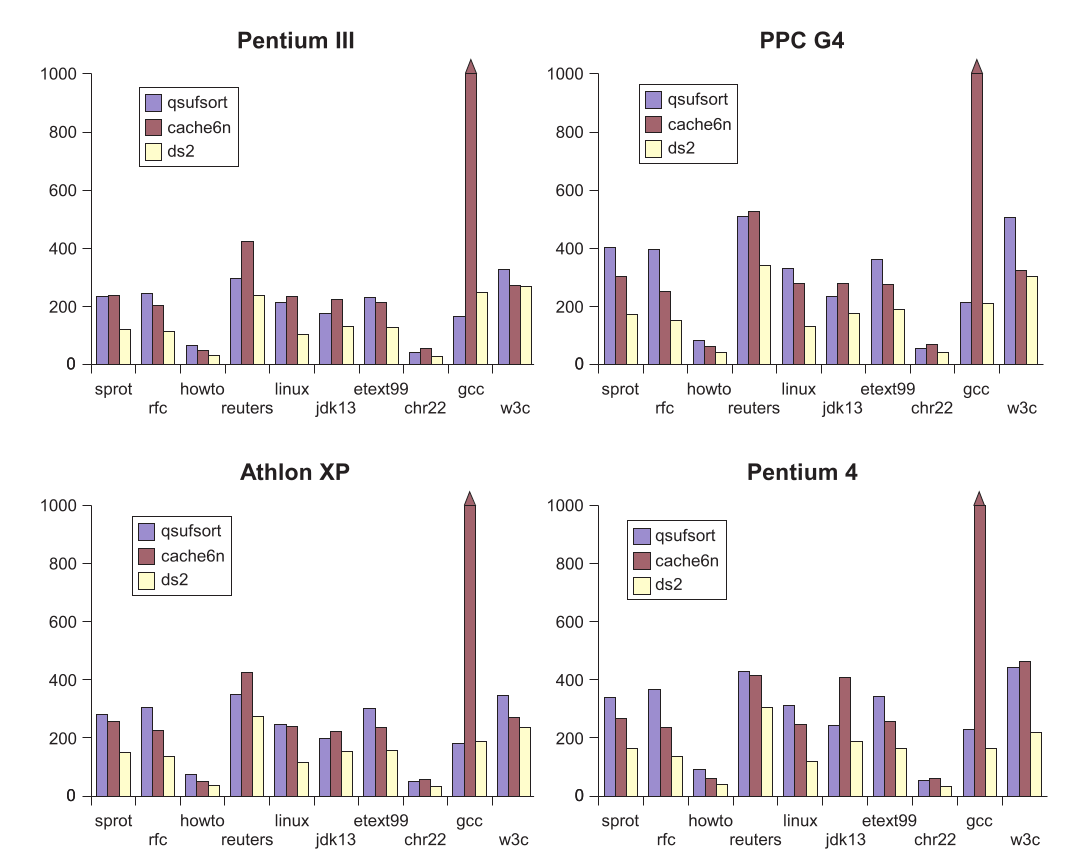
\includegraphics[width=\textwidth]{kapitel/saca_algorithmen/ds/graph.png}
\caption{Vergleich der C-Implementierung von Deep-Shallow-Sorting (ds2) mit cache~\cite{seward2000} und qsufsort~\cite{saca:1}. Abbildung von Manzini und Ferragina~\cite{saca:4}.}
\label{fg:graph}
\end{figure}

Manzini und Ferragina konnten zeigen, dass Deep-Shallow-Sorting ein zuverlässiger Ansatz ist, der mit anderen Verfahren mithalten kann~\cite{saca:4}.
Durch das Testen des Algorithmus auf vier verschiedenen (zur Zeit der Veröffentlichung aktuellen) Architekturen, Pentium III, Pentium IV, Athlon XP und PowerPC G4 haben die Autoren gezeigt, dass der Algorithmus nicht nur von einer bestimmten Plattform profitiert.
Sie vergleichen Deep-Shallow-Sorting mit \qsufsort~\cite{saca:1} und einer speichereffizienteren Variante von \cache~\cite{seward2000}. Siehe dazu Abbildung \ref{fg:graph}.
Es ist zu erkennen, dass Deep-Shallow-Sorting auf jeder der vier Architekturen und auf jedem getesteten Benchmark besser abschneidet als die anderen Algorithmen.
Zu beachten ist, dass beide verglichenen Algorithmen einen höheren Speicherbedarf als Deep-Shallow-Sorting haben.
Sie konnten zeigen, dass Deep-Shallow-Sorting ein praktischer Ansatz ist, welcher mit niedrigerem Platzverbrauch als alle verglichenen Algorithmen in fast allen Problemen eine bessere Laufzeit erreichte.

Im Laufe des ersten Semesters der Projektgruppe war es Deep-Shallow einfach möglich, die meisten Algorithmen in ihrem Speicherverbrauch zu unterbieten.
Allerdings zeigte er sich schwerfällig, die anderen Algorithmen in ihrer Laufzeit zu schlagen.
Unsere Implementierung ist immer noch weit von der Referenzimplementierung entfernt, was darauf schließen lässt, dass diese weitere Verbesserungen vornimmt, als das Paper beschreibt.

Im nächsten Semester werden wir versuchen, den Algorithmus durch Multi-Threading zu beschleunigen:
Die relativ simple Struktur des Algorithmus macht es einfach die Aufgaben auf mehrere Kerne zu verteilen.
Synchronisierung ist nur für \texttt{OFFSET}/\texttt{ANCHOR} nötig.
